\documentclass[11pt,letterpaper]{article}
\usepackage{array}
\usepackage{fullpage}
\usepackage{verbatim}
\usepackage{parskip}
\usepackage{graphicx}
	\usepackage{xcolor,colortbl}
	\definecolor{gray}{rgb}{0.95,0.95,0.95}
	\newcommand{\gray}{\cellcolor{gray}}  %{0.9}
\usepackage[flushmargin]{footmisc}

%%%%%%%%%%%%%%%%%%%%%%%%%%%%%%%%%%%%%%%%%%%%
\usepackage{termcal}
% Few useful commands (our classes always meet either on Monday and Wednesday 
% or on Tuesday and Thursday)

\newcommand{\MTWFClass}{%
\calday[Monday]{\classday} % Monday
\calday[Tuesday]{\classday} % Tuesday
\calday[Wednesday]{\classday} % Wednesday
\skipday % Thursday (no class)
\calday[Friday]{\classday} % Friday 
\skipday\skipday % weekend (no class)
}

\newcommand{\holiday}[2]{%
\options{#1}{\noclassday}
\caltext{#1}{#2}
}

\newcommand{\lab}[2]{%
\options{#1}{\noclassday}
\caltext{#1}{#2}
}


\renewcommand{\calprintdate}{%
     \ifnewmonth\framebox{\arabic{month}/\arabic{date}}%
     \else\arabic{month}/\arabic{date}%
     \fi}
         
%%%%%%%%%%%%%%%%%%%%%%%%%%%%%%%%%%%%%%%%%%%%
\renewcommand{\thefootnote}{\fnsymbol{footnote}}

\newcommand{\squeezeup}{\vspace{-2.5mm}}
\setlength{\parindent}{0in}
\newcommand{\tablespace}[0]{\vspace{8pt}}

\begin{document}
\begin{centering}
\textbf{PHYS S123: College Physics I}

Fall 2021\\
%Last updated: 9/9/19
\hspace{1cm}\\

\bigskip
\begin{table}[h]
\centering
\setlength{\extrarowheight}{2pt}
\squeezeup
\begin{tabular}{@{}r@{\hspace{0.1in}}p{4.25in}} 
{\bf Instructor:} & Jason Amundson\\
& 225 Whitehead Building\\
& jmamundson@alaska.edu\\
& phone: 796-6247 \tablespace\\
{\bf Class hours:} & MWF 10:45 am -- 11:45 am, Egan Wing 218\tablespace\\
{\bf Lab hours:} & J01, T 8:45 am -- 11:45 am, Whitehead 101\\
& J02, T 1:15 pm -- 4:15 pm, Whitehead 101\tablespace\\
{\bf Office hours:} & MWF 9:30 am -- 10:30 am, or by appointment\tablespace\\
{\bf Website:} & A course website will be maintained on Blackboard (http://classes.alaska.edu). Check for assignments, handouts, grades, and messages.\tablespace\\
{\bf Prerequisites:} & MATH S152\tablespace\\
{\bf Textbook:} & College Physics: A Strategic Approach (4\textsuperscript{th} ed.) by Knight, Jones, and Field. Be sure to purchase a version of the book that comes with an access card for MasteringPhysics, which you will use for homework submissions.
%\tablespace\\
%& The cheapest option is to purchase the MasteringPhysics with Pearson eText package (ISBN-13: 978-0-13-470235-3). If you prefer, you can also order a package that includes a bound copy of the textbook (ISBN-13: 978-0-13-464149-2). 
\tablespace\\
& When you register for the MasteringPhysics course that I have set-up, you will need to use the Access Code that you purchased and enter the course ID: amundson13945.\tablespace\\
{\bf Other materials:} & A basic, simple scientific calculator with trigonometric, exponential, and logarithmic functions. Calculators can be used during exams.
\end{tabular}
\end{table}
\end{centering}

\textbf{Student Learning Outcomes}\\
Upon successful completion of this course, students will be able to:
\begin{enumerate}\itemsep -5pt
\item Demonstrate an understanding of the basic laws of physics in classical mechanics and thermodynamics.
\item Apply these physics laws to understand physical phenomena and technological applications.
\item Demonstrate quantitative physics problem solving skills through the application of algebra and critical physics thinking.
\item Describe the societal relevance of physics and its connection to other fields of science.
\item Safely use basic laboratory equipment, develop a testable hypothesis, systematically collect and analyze data, and report and interpret experimental results.
\end{enumerate}\bigskip

Physics is the study of matter and its motion through space and time. In PHYS S123 we will cover the field of classical mechanics, which pertains to ``large'' objects that are moving much slower than the speed of light.

\bigskip
\
\begin{figure}[h]
\begin{center}
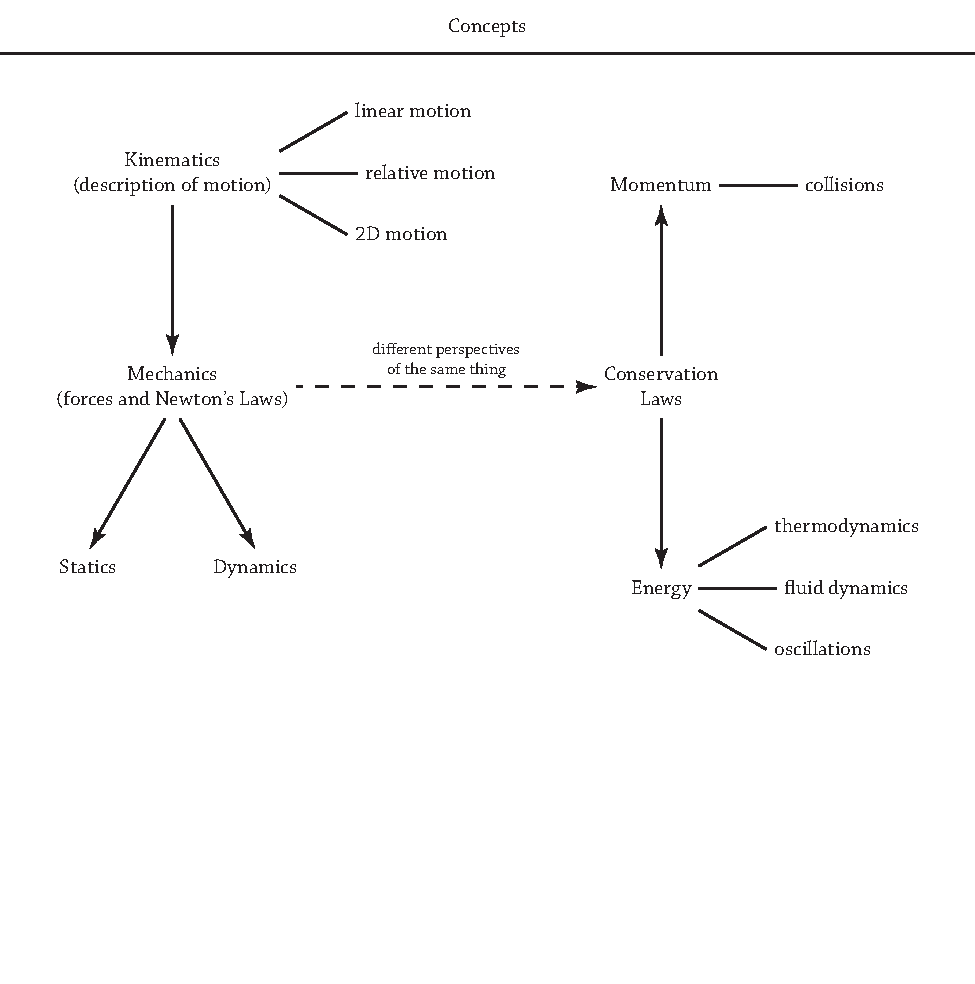
\includegraphics[width=6.5in]{./flowchart.pdf}
\end{center}
\end{figure}

\clearpage
\textbf{Grading} 
\begin{table}[h!]
\squeezeup
\begin{tabular}{ll}
Homework assignments & 20\%\\
Informal lab reports (8) & 20\%\\
Formal lab reports (2) & 15\%\\
Exams (3) & 45\%
\end{tabular}
\end{table}

Most scientific projects are collaborative; this course is no different. I encourage you to work together on homework assignments and laboratory exercises. %However, you must submit the assignments informal lab reports individually, and formal lab reports must be written individually. %Copying will not be tolerated and will result in a 0 for the assignment or report. %And anyway, cheating on the homework probably won't help your final grade since this will cause you to do more poorly on the exams.

There will be 10 homework assignments consisting of roughly 10 problems each. You will submit your solutions through MasteringPhysics. Late assignments will only be accepted for extenuating circumstances.

Why use MasteringPhysics?
\begin{itemize}\itemsep -5pt
\item It gives you wrong-answer feedback and hints for solving problems.
\item It provides me with diagnostics on what types of problems are giving you the most trouble.
\end{itemize}

A few suggestions for working through the homework:
\begin{itemize}\itemsep -5pt
\item Work through your answers slowly and be sure to check for significant figures before entering your solution. You might consider solving all of the problems before entering your answers so that you don't get frustrated right away.
\item If you feel confident in your answer, but MasteringPhysics tells you that your answer is incorrect and doesn't give you useful feedback, come talk to me or send me an e-mail. View this as an opportunity to figure out what you did wrong and correct your mistake before the due date, which is an option that you wouldn't have with paper submissions.
\item I view the homework as training for the exams and therefore I'm willing to help you work through problems all the way to the final solution if you are having trouble. 
\end{itemize}

There will also be 10 laboratory exercises during the semester. You will be expected to turn in informal reports for eight of the exercises and formal reports for two of the exercises. The informal reports may be written as a group but each person should submit the report through Blackboard. Formal lab reports must be written individually. The reports will be due one week after the lab exercises unless otherwise noted. Lab reports will not be considered late up until the point that I grade them; afterwards they will be given a maximum grade of 50\%. This late policy is designed to (1) encourage you to finish your reports even if they were not completed before the due date and (2) simplify my grading. I don't like taking off points for late work, especially if I am slow at grading it, but it is also much easier to grade everybody's work at once. I think this policy is a good compromise.\\

\clearpage
\textbf{Grading Scale}
\begin{table}[h!]
\squeezeup
\begin{tabular}{ll}
A & 93--100\% \\
A- & 90--92\% \\
B+ & 87--89\% \\
B & 83--86\% \\
B- & 80--82\% \\
C+ & 77--79\% \\
C & 73--76\% \\
C- & 70--72\% \\
D+ & 67--69\% \\
D & 63--66\% \\
D- & 60--62\% \\
F & $<$60\%
\end{tabular}
\end{table}

\textbf{General Comments}\\
My job is to help you learn. If you are uncomfortable in the classroom or have any other comments and concerns, please do not hesitate to contact me.

When I'm in the office I'll try to respond to your phone calls and e-mails as quickly as possible. Any messages sent to me in the evening or on weekends will likely not be addressed as quickly.\\

%\textbf{Conduct}\\
%Please turn off cell phones, laptops, and other electronic devices (except calculators) during lecture unless you need them to aid. They can be a distraction to you and your fellow students.\\

\textbf{Student Ratings of Instruction}\\
During the last three weeks of class, you will have an opportunity to complete an online rating questionnaire on course instruction, how the course aided in your skill development,  effectiveness of technology and equipment used, and adequacy of library resources and services used during the course. You will receive notification in your UAS email account when the rating questionnaire is available. Please make use of this opportunity to provide feedback on what worked for you and what did not. Your input is used to assess methods and services in order to provide the best educational experience possible.\\

\textbf{Disabilities}\\
If you experience a disability and would like information about support services, please contact Disability Support Services, located at the Student Resource Center in the Mourant building.  They can be reached at 796-6000. For more information, please see http://www.uas.alaska.edu/dss/index.html.\\

\textbf{Title IX/Sexual Misconduct}\\
All students have the right to be free from all forms of gender and sex-based misconduct (sexual harassment, dating violence, domestic violence, sexual assault, or stalking). Please report any incidence of sex or gender-based discrimination to the UAS Title IX Office: 796-6371 or email {uas.title9@alaska.edu}. More information and resources are available at\\ http://www.uas.alaska.edu/policies/titleix.html.

\clearpage
\paragraph*{Schedule (subject to change):}
\begin{center}
\begin{calendar}{8/23/2021}{16} 
% Semester starts on 8/23/2021 and lasts for 16
% weeks, including finals week

\setlength{\calboxdepth}{.6in}
\renewcommand{\calprintclass}{}
\MTWFClass

% August
\caltexton{1}{Course overview: why physics?}
\caltextnext{1.1--1.6: Introduction to kinematics}
\caltextnext{2.1--2.6: Kinematic equations}
\caltextnext{3.1--3.3, 3.5: Motion in two dimensions}

% September
%\caltextnext{\gray TBD}

\caltextnext{\gray 3.4--3.6: Motion in two dimensions, ctd.\\{\bf HW \#1 due}}
\caltextnext{\gray 3.8: Relative motion}
\caltextnext{\gray 3.7, 6.1: Circular motion\\{\bf HW \#2 due}}

\caltextnext{\gray 7.1--7.2: Rotational motion}
\caltextnext{\gray Circular and rotational motion, ctd.}


\caltextnext{\gray 4.1--4.7: Newton's Laws}
\caltextnext{\gray 5.3--5.4, 5.8, 6.6: Types of forces, I\\{\bf HW \#3 due}}
\caltextnext{\gray {\bf Exam \#1}\\Testing Center}

\caltextnext{\gray 5.5: Types of forces, II}

\caltextnext{\gray 5.6, 8.3: Types of forces, III}
\caltextnext{6.3--6.4, 6.6: Centripetal forces}


\caltextnext{7.3--7.4: Torque}
\caltextnext{7.5--7.7: Torque, II\\{\bf HW \#4 due}}
% October
\caltextnext{8.1--8.2 Static equilibrium}

\caltextnext{8.4: Equilibrium and elasticity}
\caltextnext{9.1--9.3: Impulse and momentum\\{\bf HW\#5 due}}
\caltextnext{9.4--9.6: Conservation of momentum}

\caltextnext{9.7: Angular momentum}
\caltextnext{10.1--10.2: Work and energy\\{\bf HW\#6 due}}
\caltextnext{10.3--10.5: Types of energy}

\caltextnext{10.6--10.7: Types of energy, II}
\caltextnext{11.1, 11.4--11.7, 12.5: Introduction to thermodynamics\\{\bf HW \#7 due}}
% November
\caltextnext{{\bf Exam \#2}\\Testing Center}

\caltextnext{\gray 12.6: Applications of thermodynamics}
\caltextnext{\gray 12.8: Heat transfer}
\caltextnext{\gray 12.2--12.4, 12.7: Thermodynamics of gases}

\caltextnext{\gray 13.1--13.2: Introduction to fluids}
\caltextnext{\gray 13.3: Archimedes' principle\\{\bf HW \#8 due}}
\caltextnext{\gray 13.4--13.5: Fluid dynamics, I}

\caltextnext{\gray 13.6--13.7: Fluid dynamics, II}
\caltextnext{\gray 14.1--14.5: Oscillations\\{\bf HW \#9 due}}

\caltextnext{\gray 14.6--14.7: Driven and damped oscillations}
\caltextnext{\gray 15.1--15.3: Introduction to waves}
\caltextnext{\gray 15.4--15.7: Traveling waves}

% December
\caltextnext{16.1--16.3: Wave superposition}
\caltextnext{16.4--16.5: Sound\\{\bf HW \#10 due}}


% Field work
\holiday{9/15/2021}{\gray No class (tentative)}
\holiday{9/17/2021}{\gray No class (tentative)}

% Labs
\lab{8/24/2021}{Lab \#1: Measurements and motion}
\lab{8/31/2021}{Lab \#2: Acceleration\\{\bf Lab \#1 due}}

\lab{9/7/2021}{\gray Lab \#3: Forces\\{\bf Lab \#2 due}}
\lab{9/14/2021}{\gray No lab (tentative)}
\lab{9/21/2021}{\gray Review for exam \#1}
\lab{9/28/2021}{\gray Lab \#4: Circular motion (formal report)\\{\bf Lab \#3 due}}

\lab{10/5/2021}{Lab \#5: Torque \\{\bf Lab \#4 due}}
\lab{10/12/2021}{Lab \#6: Statics \\{\bf Lab \#5 due}}
\lab{10/19/2021}{Lab \#7: Momentum and energy\\{\bf Lab \#6 due}}
\lab{10/26/2021}{Review for exam \#2}

\lab{11/2/2021}{\gray Lab \#8: Springs (formal report)\\{\bf Lab \#7 due}}
\lab{11/9/2021}{\gray No lab}
\lab{11/16/2021}{\gray Lab \#9: Pendulums\\{\bf Lab \#8 due}}
\lab{11/23/2021}{\gray Lab \#10: Sound\\{\bf Lab \#9 due}}
\lab{11/30/2021}{\gray Review for exam \#3\\{\bf Lab \#10 due}}

% Holidays
\holiday{9/6/2021}{\gray Labor Day}
\holiday{11/24/2021}{\gray No class}
\holiday{11/25/2021}{\gray Thanksgiving holiday}
\holiday{11/26/2021}{\gray Thanksgiving holiday}
\holiday{12/6/2021}{{\bf Exam \#3}\\ Testing Center}


\end{calendar}
\end{center}


\end{document}
